% !TeX spellcheck = en_US
\documentclass[12pt, a4paper]{report}
\usepackage[scaled]{helvet}
\renewcommand\familydefault{\sfdefault}
\usepackage[T1]{fontenc}
\usepackage[margin=0.5in]{geometry}
\usepackage{float}
\usepackage{framed}
\usepackage{multicol}
\usepackage{amsmath}
\usepackage{amssymb}
\usepackage[framemethod=TikZ]{mdframed}
\usepackage{graphicx}
\usepackage{enumitem}
\usepackage{gensymb}
\setlist{nosep}
\usepackage{booktabs}
\usepackage{makecell}
\usepackage{tikzsymbols}
\usepackage{hyperref}
\hypersetup{
	colorlinks,
	citecolor=black,
	filecolor=black,
	linkcolor=black,
	urlcolor=black
}
\usepackage{multirow}
\usepackage{pgf-umlsd}
\usepackage{soul}
\usepackage{pgfplots}
\usepackage{tikz}
\usepackage{circuitikz}
\tikzstyle{dot} = [shape=circle, fill=black]
\usepackage{tikz-timing}
\usetikzlibrary{arrows,shapes,automata,petri,positioning,calc}
\tikzset{
	place/.style={
		circle,
		thick,
		draw=black,
		fill=white,
		minimum size=6mm,
	},
	state/.style={
		circle,
		thick,
		draw=blue!75,
		minimum size=6mm,
	},
}
%\usepgfplotslibrary{external}
%\tikzexternalize

\newcounter{note}\setcounter{note}{0}
\renewcommand{\thenote}{\arabic{note}}
\newenvironment{note}[1]{
	\begin{minipage}{0.9\linewidth}
		\vspace{1em}
		\stepcounter{note}
		\ifstrempty{#1}{
			\mdfsetup{
				frametitle={
					\tikz[baseline=(current bounding box.east),outer sep=0pt]
					\node[anchor=east,rectangle,fill=blue!20]
					{\strut Note~\thenote};
				}
			}
		}{
			\mdfsetup{
				frametitle={
					\tikz[baseline=(current bounding box.east),outer sep=0pt]
					\node[anchor=east,rectangle,fill=blue!20]
					{\strut Note~\thenote:~#1};
				}
			}
		}
		\mdfsetup{innertopmargin=0pt,linecolor=blue!20,linewidth=2pt,topline=true,frametitleaboveskip=\dimexpr-\ht\strutbox\relax}
		\begin{mdframed}[]\relax
		}{
	\end{mdframed}\end{minipage}
}
\newenvironment{code}{\ttfamily}{\par}

\begin{document}
	\tableofcontents
	\vspace{2em}
	\textbf{Contributors:}
	\begin{itemize}
		\item Daniel Fitz (Sanchez)
	\end{itemize}
	\section{Assessment}
	\begin{itemize}
		\item Online Quizzes (10\% = Best 10 $\times$ 1\%)
		\subitem Due Mondays at 8am
		\item Mid-semester exam (10\% or 20\%)
		\subitem Saturday (centrally scheduled - sometime week 5 to 7)
		\subitem Multiple-choice, open-book
		\item Prac Exam (Pass/Fail)
		\subitem Held during Monday/Wednesday Learning Lab sessions in week 6
		\subitem You must pass in order to pass the course
		\item Project (20\%)
		\subitem Develop a microcontroller program
		\item Final Exam (50\% or 60\%)
		\subitem Short answer, problem solving, open-book
	\end{itemize}

	\newpage

\begin{multicols}{2}

\chapter{Lecture Notes}
% !TeX spellcheck = en_US
% !TeX root = notes.tex
\section{Bits, Bytes and Binary}
\subsection{Structured Computer Organization}
\begin{description}
	\item[Level 5:] Problem-oriented language level
	\item[Level 4:] Assembly language level
	\item[Level 3:] Operating system machine level
	\item[Level 2:] Instruction set architecture level
	\item[Level 1:] Microarchitecture level
	\item[Level 0:] Digital Logic level
\end{description}

\subsection{Unsigned Number in Binary}
Each bit position has a value $\rightarrow 2^n$ (starting at zero). Add all values of the positions together and that's unsigned value.

\subsection{Converting Decimal to Binary}
\begin{itemize}
	\item Method 1
	\subitem rewrite $n$ as sum of powers of 2 (by repeatedly subtracting largest power of 2 not greater than $n$)
	\subitem Assemble binary number from 1's in bit positions corresponding to those powers of 2, 0's elsewhere
	\item Method 2
	\subitem Divide $n$ by 2
	\subitem Remainder of division (0 or 1) is next bit
	\subitem Repeat with $n$ = quotient
\end{itemize}

\begin{note}{Example}
	Convert 53 to binary
	\begin{align*}
		\frac{53}{2} &= 26 \text{ rem } 1 \Rightarrow 1\\
		\frac{26}{2} &= 13 \text{ rem } 0 \Rightarrow 0\\
		\frac{13}{2} &= 6 \text{ rem } 1 \Rightarrow 1\\
		\frac{6}{2} &= 3 \text{ rem } 0 \Rightarrow 0\\
		\frac{3}{2} &= 1 \text{ rem } 1 \Rightarrow 1\\
		\frac{1}{2} &= 1 \text{ rem } 1 \Rightarrow 1
	\end{align*}
	$\therefore 53 \equiv 0b110101$
\end{note}

\subsection{Least and Most Significant Bits}
\begin{description}
	\item[Most Significant Bit (MSB):] Bit that's worth the most, the left-most bit
	\item[Least Significant Bit (LSB):] Bit that's worth the least, the right-most bit
\end{description}

\begin{note}{Radices}
	\begin{itemize}
		\item \textbf{Radix:} number system base
		\item A radix-k number system
		\subitem $k$ different symbols to represent digits 0 to $k-1$
		\subitem Value of each digit is (from the right) $k^0, k^1, k^2, k^3, \ldots$
		\item Often convenient to deal with
		\subitem\textbf{Octal} (radix-8) - Symbols: 0, 1, 2, 3, 4, 5, 6, 7
		\subsubitem\textit{One octal digit corresponds to 3 bits}
		\subitem\textbf{Hexadecimal} (radix-16) - Symbols: 0, 1, 2, 3, 4, 5, 6, 7, 7, 8, 9, A, B, C, D, E, F
		\subsubitem\textit{One hexadecimal digit corresponds to 4 bits (useful)}
	\end{itemize}
\end{note}

\begin{note}{Radix Identification}
	\begin{itemize}
		\item Hexadecimal
		\subitem Leading 0x (C, Atmel AVR)
		\subitem Trailing h (Some assembly languages)
		\subitem Leading \$ (Atmel AVR Assembly)
		
		\item Octal
		\subitem Leading 0 (C, Atmel AVR)
		\subitem Trailing q (Some assembly languages)
		\subitem Leading @ (Some assembly languages)
		
		\item Binary
		\subitem Leading 0b (Atmel AVR Assembly, Some C)
		\subitem Trailing b (Some assembly languages)
		\subitem Leading \% (some assembly languages)
	\end{itemize}
\end{note}
% !TeX spellcheck = en_US
% !TeX root = notes.tex
\subsection{Conversions}
Easiest to convert from most formats to binary then to the desired format.

\subsubsection{Octal}
\begin{description}
	\item[From Binary:] Group bits into series of 3 and then convert to decimal (0b010 = 02)
	\item[To Binary:] Convert each octal number to binary and append
\end{description}

\subsubsection{Hex}
\begin{description}
	\item[From Binary:] Group bits into series of 4 and then convert to hex with overflow being apart of the alphabet (0b1100 = 0xC)
	\item[To Binary:] Convert each hex number to binary and append
\end{description}

\subsubsection{Decimal}
\begin{description}
	\item[From Binary:] Add together the powers of two at each position $n$ ($0b1010 = 2^3 + 2^1 = 10$)
	\item[To Binary:] Starting with LSB, divide by 2 with the remainder being bit value at position. ($9 = 9/2 = 4 rem 1, 4/2 = 2 rem 0, 2/2 = 1 rem 0, 1/2 = 0 rem 1. \therefore 9 = 0b1001$)
\end{description}


\subsection{Negative Numbers}
\subsubsection{Signed Magnitude}
Leftmost bit is the sign bit, true is negative and false is positive

\subsubsection{One's Complement}
Leftmost bit = sign-bit (as per signed magnitude), true is negative and false is positive. If negative all bits are inverted

\subsubsection{Two's Complement}
MSB signifies if negative, true is negative and false is positive. To negate invert all bits and add decimal 1.
\begin{leftbar}
	Allows addition without requiring conversion	
\end{leftbar}


\subsubsection{Excess $2^{m-1}$}
e.g. for 8 bits, excess-128. Add 128 to the original bit and convert to binary
% !TeX spellcheck = en_US
% !TeX root = notes.tex
\section{Lecture 2: Bitcoin, Cryptocurrencies Blockchain Technology}
Blockchain is over-hyped!
\subsection{Blockchain (or Hash Chain/List)}
\begin{itemize}
	\item Use hash pointers to build structures similar to a linked list
	\item Head hash pointer of the list protects the integrity of the entire list or chain (Need to store hash pointer to the head of the list externally to list)
	\item Hash is computed over entire block, including header, which includes hash pointer to previous block
	\item First block is called \textbf{Genesis Block}
	\item If an attacker modifies a block, they need to modify the contents of all subsequent blocks
\end{itemize}
\subsubsection{Merkle Trees}
\begin{note}{Merkle Trees}
	\begin{itemize}
		\item Named after Ralph Merkle
		\item Can protect integrity of large number of data blocks, like a Blockchain
		\item We only need the \textbf{Root Hash} at the root of the tree (\textbf{Merkle Root})
		\item Modification of any data block by attack results in different hashes all the way up to the Merkle Root, and can easily be detected
		\item Cost to prove \texttt{Tx1} in the tree: $O(\log_2 N)$
	\end{itemize}
\end{note}
\begin{figure}[H]
	\includegraphics[width=\linewidth]{merkle}
	\centering
	\caption{Merkle Tree Layout}
\end{figure}
\subsubsection{Use of Merkle Trees in Bitcoin}
Bitcoin uses Merkle Trees to store Transactions in a ``Block'' ($\approx2000$)
\begin{itemize}
	\item Each Block stores a \textbf{Merkle Root}
	\item Merkle Trees allow verification that a transaction is part of a Block without having the entire block, only Merkle Path is required. This is used to implement Simplified Payment Verification (SPV) in Bitcoin
\end{itemize}
Blocks are then stored in a Blockchain

\subsection{Public Key Cryptography -- Digital Signatures}
Properties of signatures
\begin{itemize}
	\item Only \textbf{you} can provide a valid signature, anyone can verify
	\item Signature is tied to a particular document, cannot be copy-pasted to another document
\end{itemize}
Public Key Cryptography
\begin{itemize}
	\item Asymmetric operation
	\item Two keys: Public key and Private key
\end{itemize}
Encryption
\begin{itemize}
	\item Encryption with Public Key
	\item Decryption with Private Key
	\item Key Benefit: Simplified key distribution/management
	\item Remaining security problems $\rightarrow$ Authenticity of public key, Public Key Certificates (map public key to identity)
\end{itemize}
Digital Signature
\begin{itemize}
	\item Sign with Private Key
	\item Verification with Public Key
\end{itemize}
\begin{leftbar}
	Since public key operations are computationally expensive, digital signatures are typically applied to a hash, rather than entire file or block of data
\end{leftbar}
\subsubsection{Digital Signatures in Bitcoin}
Bitcoin transactions have digital signatures
\begin{itemize}
	\item Signed by the owner(s) of the source funds (Bitcoin to be transferred)
	\item This proves ownership of funds
	\item Prevents forgery of coins/transactions
\end{itemize}
\begin{note}{Bitcoin Identity}
	An identity in Bitcoin (a \textbf{Bitcoin Address}) is simply a public key (160-bit hash of it, to be precise)
	\begin{itemize}
		\item No need for public key certificates
		\item No need to link public key to a real name
	\end{itemize}
\end{note}

\subsubsection{Hashcash}
\begin{note}{Hashcash}
	Prevent of mitigate \textbf{denial-of-service} (DoS) attacks by requiring the sender to solve a puzzle before connecting
	\begin{sequencediagram}
		\newinst{c}{Client}
		\newinst[3]{s}{Server}
		
		\mess{c}{Request Service}{s}
		\mess{s}{Choose Challenge}{s}
		\mess{s}{Send Challenge}{c}
		\mess{c}{Solve}{c}
		\mess{c}{Response}{s}
		\mess{s}{Verify}{s}
		\mess{s}{Grant Service}{c}
	\end{sequencediagram}
\end{note}
\begin{itemize}
	\item Require the first $n$ bits of $h(x)$ to have a given value, first $n$ bits are all $0$ (partial pre-image)
	\item Same as saying $h(x) < T$
	\item Best approach is brute forcing
	\item Chance of guessing on single try: $2^{-n}$, expected number of tries until success: $2^n$
\end{itemize}
\textit{Bitcoin aims to have a block solved roughly every 10 minutes, difficulty is adjusts every 2016 blocks ($\approx2$ weeks)}

\subsection{Cryptocurrency}
\begin{description}
	\item[Broadcasting of transactions:] Unstructured P2P Network, flooding (as used in Bitcoin)
	\item[Avoiding forgery (transactions, coins):] Digital Signatures
	\item[Maintaining the public ledger:] P2P Network, Proof-of-work and Incentive mechanism
\end{description}
% !TeX spellcheck = en_US
% !TeX root = notes.tex
\section{Lecture 3: Bitcoin, Cryptocurrencies Blockchain Technology}
\subsection{Sybil Attack}
\begin{itemize}
	\item Named after the subject of the book \textbf{Sybil}, a case study of a woman diagnosed with multiple personality disorder
	\item Such fals identities are called \textbf{``Sybils''}, in the context of P2P systems
	\item Or \textbf{``Sockpuppets''} in the context of the Internet, e.g. to manipulate public opinion
	\begin{leftbar}
		``... referred to a false identity assumed by a member of an Internet community who spoke to, or about, themselves while pretending to be another person. `The term now includes other misleading uses of online identities, such as those created to praise, defend or support a person or organization, to manipulate public opinion, or to circumvent a suspension or ban from a website''\\
		- Wikipedia
	\end{leftbar}
\end{itemize}

\subsection{Decentralized Consensus in Bitcoin}
\begin{itemize}
	\item Bitcoin achieves consensus by replacing \textbf{one node (or one IP address) one vote}, with \textbf{one CPU one vote}
	\item Bitcoin mining uses mostly ASICs and GPUs, not CPUs
	\item Consensus is achieved by a (probabilistic) majority vote, based on computing power
	\begin{itemize}
		\item Attacker needs > 50\% of combined computing power in order to cheat with high probability
		\item This is harder to achieve than controlling more than half of the nodes
		\item It's relatively easy to spin up a few thousand VMs as nodes, compared to controlling >50\% of Bitcoin's mining compute power
	\end{itemize}
	\item Bitcoin combines a \textbf{proof-of-work mechanism} (based on Hashcash), combined with a clever incentive mechanism $\rightarrow$ Nodes get paid to do the right thing, i.e. checking and confirming valid transactions via ``mining''
\end{itemize}

\section{Lecture 3: Bitcoin}
\begin{itemize}
	\item Complete transaction history is stored in public ledger (blockchain), stored by nodes in P2P network
	\item New transactions are created off-line, and then broadcast is P2P network
	\item Nodes validate and relay transactions (if valid)
	\item Nodes add new transactions (not part of blockchain yet) to a \textbf{transaction pool}
	\item Nodes combine transactions in pool to a block, and try to solve the corresponding proof-of-work puzzle, to ``confirm'' the block
	\item Node that finds solution first broadcasts block with solution in the network (Winning node selection is probabilistic, with probability propertional to computing power)
	\item Nodes check solution, and if OK, add new block to their local copy of blockchain
	\item All nodes who were working on solving the old puzzle, immediately start working on a new block
	\begin{itemize}
		\item Everybody always works on the longest chain
		\item Convergence to longest chain provides consensus
		\item Forks happen but are resolved by (computational) majority vote
	\end{itemize}
\end{itemize}
\begin{note}{Bitcoin Components}
	\begin{itemize}
		\item Bitcoin Network
		\item Bitcoin Identities/Addresses
		\item Bitcoin Transactions
		\item Bitcoin Scripting Language
		\item Blocks
		\item Proof-of-work, Hash puzzles, Mining
		\item Consensus
	\end{itemize}
\end{note}

\subsection{Bitcoin Network}
Transactions are broadcast in the Bitcoin network, consisting of ``full'' Bitcoin nodes ($\approx$10,000)
\begin{itemize}
	\item Best-effort (asynchronous, unreliable), it's enough if only some nodes get the message
	\item It's easy to join the Bitcoin Network, just download and run the client (Bitcoin is a \textbf{permissionless, public} blockchain, anyone can join)
\end{itemize}
Network is unstructured P2P network (random topology)
\begin{itemize}
	\item Similar to Gnutella (a P2P system from a long time ago)
	\item Overlay network, TCP, port 8333
	\item Messages are flooded
	\item All nodes are equal, no hierarchy
	\item Nodes can join at any time
	\item Node is `forgotten' if it does not respond for more than 3 hours
	\item Network is very simple and robust, e.g. to churn, but not very efficient
\end{itemize}
\begin{note}{Bitcoin Network Nodes}
	\begin{itemize}
		\item Check validity of transactions
		\item Relay transactions in the network via flooding
		\item Mining (proof-of-work puzzles)
		\item Validate and forward confirmed blocks (Add them to local copy of blockchain)
	\end{itemize}
\end{note}
\subsection{Bitcoin Identity and Addresses}
Users are represented by their Public Key addresses (hash), called \textbf{Bitcoin Addresses}, which serve as a pseudonyms
\begin{itemize}
	\item An address is a \textbf{160 bit} value, and is computed as follows
	\item RIPEMD160 hash of SHA-256 hash of ECDSA Public Key
	\item This is a ``Pay-to-pubkey-hash (P2PKH)'' address, encoding starts with ``1''
\end{itemize}
When spending a coin, spender needs to proof ownership of coin by providing a valid digital signature on the spend transaction (i.e. proving ownership of corresponding private key)\\
How can digital signatures be verified?
\begin{itemize}
	\item We need public key, not just hash of public key
	\item Spender of coin needs to provide both valid signature AND public key
	\item How do we know the provided public key is authentic $\rightarrow$ Hash it, and compare with Bitcoin address, which is the hash of public key
\end{itemize}
Bitcoin also supports \textbf{Pay to script hash (P2SH)} addresses
\begin{itemize}
	\item Allow transactions to be sent to a \textbf{script hash} instead of a public key hash (Address encoding starts with a `3' instead of `1')
	\item To spend bitcoins sent via P2SH, the recipient must provide a script matching the script hash and data which makes the script evaluate to true
	\item Allows more complex transactions (\textbf{smart contracts}), e.g. transaction outputs that require multiple signatures (multisig), or transaction puzzle, ...
\end{itemize}
\begin{note}{Bitcoin Address Encoding}
	Bitcoin uses Base58 encoding (binary-to-text encoding). Similar to Base64 encoding, but without some characters. Rationale, as explained in original bitcoin client source code:
	\begin{code}
		// Why base-58 instead of standard base-64 encoding?\\
		// - Don't want 0OIL characters that look like the same in some fonts and\\
		//   could be used to create visually identical looking account numbers.\\
		// - A string with non-alphanumeric characters is not as easily accepted as an account nbr.\\
		// - E-mail usually won't line-break if there's no punctuation to break at.\\
		// - Doubleclicking selects the whole number as one word if it's all\\alphanumeric.
	\end{code}
	Bitcoin also adds 4 byte checksum to addresses
\end{note}
\subsubsection{Bitcoin Address -- Balance}
\begin{itemize}
	\item The ``balance'' of an address is the total of unspent transaction outputs (UTXO) sent to the address.
	\item ``There are no accounts or balances in bitcoin; there are only unspent transaction outputs (UTXO) scattered in the blockchain''
	\item A user typically has many different addresses, all managed by the ``wallet'' software
	\item The wallet ``balance'' is the sum of all unspent transaction outputs of all addresses owned by the user
\end{itemize}
\subsection{Bitcoin Transactions}
\begin{itemize}
	\item Transaction are created off-line (No need to be connected to Bitcoin network for this)
	\item Transactions are broadcast in Bitcoin P2P network
	\item Nodes check validity, and relay transaction (flooding)
	\item Nodes add to new transactions to a block and try to solve hash puzzle
	\item A block with a solved puzzle is ``confirmed'', and broadcast in the network, and added to the blockchain of each node
	\item Contains:
	\begin{itemize}
		\item Inputs (any number $\geq0$)
		\item Outputs (any number > 0)
		\item Digital signatures of input coin owners (Typically for \textbf{P2PKH} transactions)
		\item Input needs to be completely consumed (With exception of Transaction Fee)
	\end{itemize}
\end{itemize}
\subsubsection{Basic Transaction Types}
\begin{itemize}
	\item Common Transaction
	\begin{itemize}
		\item 1 input
		\item 1 ``normal'' output
		\item 1 change output (back to owner)
		\subitem Create new ``Change Address' to maintain ``anonymity''
	\end{itemize}
	\item Aggregating Transaction
	\begin{itemize}
		\item Multiple inputs
		\item 1 output
	\end{itemize}
	\item Distributing Transaction
	\begin{itemize}
		\item 1 input
		\item Multiple outputs
	\end{itemize}
	\item ``Coinbase Transaction''
	\begin{itemize}
		\item 0 input, 1 outputs
		\item Freshly created (``minted'') coins
		\item Miner gets this as a reward for solving Hash puzzle (and thereby confirming block)
		\item First transaction in every block
	\end{itemize}
\end{itemize}

\subsection{Bitcoin Scripts}
\begin{itemize}
	\item Two types of Bitcoin scripts to validate transactions
	\begin{itemize}
		\item a locking script (Typically \textbf{ScriptPubKey})
		\item and an unlocking script (Typically \textbf{ScriptSig})
	\end{itemize}
	\item A locking script is a condition placed on an output
	\item It specifies the conditions that must be met to spend or consume the output in the future
	\begin{itemize}
		\item Typically a \textbf{valid digital signature} of the claimed owner
		\item Can be other things, to implement basic `smart contracts'
	\end{itemize}
\end{itemize}
\subsubsection{Bitcoin Scripting Language ``Script''}
\begin{itemize}
	\item Allows to program conditions required for the spending of Bitcoins (``Programmable Money'')
	\item \textbf{Script} is a simple, stack based language
	\item Not Turing complete (e.g. no loops)
	\item Scripts are guaranteed to terminate after a fixed number of steps, e.g. no infinite loops
	\item Why is this a good thing?
	\begin{itemize}
		\item Avoids potential denial of service attacks on nodes, ``logic bombs''
		\item Remember: Every node runs all scripts to validate all transactions (BTW, this severely limits scalability of Bitcoin)
	\end{itemize}
	\item In contrast, Ethereum has a Turing complete scripting language
	\subitem Solves DoS attack problem by putting a price on script computation (`Gas')
\end{itemize}

\subsection{Blocks}
\begin{itemize}
	\item Transactions are grouped into blocks
	\subitem This is an optimization. Confirming individual transactions and adding them to the blockchain would be possible, but very inefficient
	\item Transactions are stored in a Merkle Tree, with the Merkle Root (Tx\_Root) stored in the block header
	\item Once confirmed (via solving hash puzzle), a block is added to the blockchain
	\item The `Nonce' is the solution of the hash puzzle
\end{itemize}
\subsubsection{How are blocks added to the Blockchain?}
\begin{itemize}
	\item Multiple nodes (miners) are working towards solving the hash puzzle for a new block
	\subitem miners are probably working on different version of blocks, depending on content on their transaction pool
	\item First node who solves puzzle, broadcasts new block with solution (nonce) in the Bitcoin P2P network
	\begin{itemize}
		\item Choice of winning node is random (probabilistic)
		\item Probability of success is proportional to computing power of miner
	\end{itemize}
	\item ``Block Height'' is sequence number of blocks
	\item Other nodes check if solution is correct, and if so, add block to their local copy of the blockchain, and forward new block to other nodes
\end{itemize}

\subsection{Bitcoin Mining}
\begin{itemize}
	\item At the current level of difficulty, solving Bitcoin hash puzzles is hard and expensive
	\item Mostly ASICs based, some GPUs
	\item Total hash rate of entire Bitcoin network $\approx25\times10^{18}$H/s
	\item Hash rate of an Intel i7 CPU $\approx10$MH/s
	\subitem Need > 10,000,000 laptops to be able to mine one block per year on average
	\item Finite amount of BTC $\approx$21 Million
	\item Bitcoin is deflationary (value increases, people are potentially hoarding Bitcoin)
\end{itemize}
\subsubsection{Mining Incentive/Reward}
\begin{itemize}
	\item Transaction Fees
	\begin{itemize}
		\item Difference between total input and total output value of transaction
		\item Optional, but miners prioritize inclusion of transactions into blocks based on fees (Like giving a tip)
	\end{itemize}
	\item Block Reward
	\begin{itemize}
		\item For each solved puzzle (confirmation of block), miner currently gets freshly minted 12.5 BTC
		\item ``Coinbase transaction'' ($1^{st}$ transaction in each block)
		\item This is the only way in which coins are generated in Bitcoin
		\item Reward halved every 4 years (initially 50 BTC)
		\item Essentially no more Block Reward in 2040
	\end{itemize}
\end{itemize}

\subsection{Consensus}
\begin{itemize}
	\item Blockchain forks can happen, e.g. due to race conditions and variable latency in Bitcoin network (\textit{two nodes might find a solution to the puzzle at almost the same time}), or due to double spend attempt
	\item Nodes converge on one chain, they all aim to work on the longest (main) chain, and eventually one chain wins
	\item Incentive to work on the longest chain (Block Reward and TX fees can only be spent if block remains in the longest chain (need a certain number of \textbf{confirmations}, i.e. blocks added))
	\item Block on discontinued branches are called ``orphaned blocks''
	\item Heuristic
	\subitem Transactions are considered ``confirmed'' if they are in a block that has at least 6 blocks added to the chain (i.e. 6 confirmation) \textit{(There is nothing special about the number 6)}
	\item This means if someone wanted to reverse a transaction, they would have to go back 6 blocks, and re-do all the hash puzzles, before another nodes adds a new block at the end of chain (Practically impossible, unless attacker hash more than 50\% of computing power of entire network)
	\item Other types of attacks:
	\begin{itemize}
		\item Publish an invalid transaction, e.g. trying to spend coins that he does not own (no valid signature). Honest nodes would reject the transaction
		\item Double spend attack. Cause a fork in the chain, majority vote will guarantee that only one chain will exist
		\item Launch DoS attack against
	\end{itemize}
	\item With more than 50\% computing power, more beneficial to play by the rules and gain Block Rewards
\end{itemize}
% !TeX spellcheck = en_US
% !TeX root = notes.tex
\section{Navigation Systems}
\subsection{Wayfinding}
\begin{leftbar}
	``How we navigate through complex physical spaces'' - Kevin Lynch: The Image of the City (1960)	
\end{leftbar}
\begin{note}{4 Core Components of Wayfinding}
	\begin{itemize}
		\item Orientation
		\item Route decisions
		\item Mental mapping
		\item Closure	
	\end{itemize}
\end{note}
\begin{note}{5 Common Elements of Wayfinding}
	\begin{itemize}
		\item Paths
		\item Edges
		\item Districts
		\item Nodes
		\item Landmarks
	\end{itemize}
\end{note}

\subsection{Types of Navigation}
\subsubsection{Primary Navigation}
Main header menu
\subsubsection{Secondary Navigation}
Some sub heading under the main menu
\subsubsection{Supplementary Navigation}
Navigation on the side (similar to sort by category)
\subsubsection{Local Navigation}
Navigation of the headings within the current page
\subsubsection{Breadcrumbs}
Provides a hierarchy view of the current page location
\subsubsection{Utility Navigation}
Extra menus and systems hidden away but provided commonly through icons
\subsubsection{Footer Navigation}
Stuff at the bottom of the page
\subsubsection{Global/Universal Navigation}
The whole header banner, included could be:
\begin{itemize}
	\item Primary Navigation
	\item Secondary Navigation
	\item Utility Navigation
\end{itemize}

\begin{note}{What Not To Do!}
	Mystery Meat Navigation
	\begin{itemize}
		\item A visually attractive but inefficient or confusing user interface
		\item Obscures navigation
		\item Forcing user to explore (could be excused)	
	\end{itemize}
	Surprise Dropdowns
	\begin{itemize}
		\item Unclear when dropdowns are available
		\item Always indicate that there is more hidden information	
	\end{itemize}
\end{note}

\begin{note}{Good Practice Standards}
	\begin{itemize}
		\item Use familiar names for links
		\item Clearly distinguish between different types of navigation
		\item Use common positioning	
	\end{itemize}
	
\end{note}

\section{HTML Sectioning and Layout}
\subsection{HTML Sectioning Elements}
\begin{description}
	\item[section:]
	\item[article:]
	\item[aside:]
	\item[nav:]
	\item[header:]
	\item[footer:]	
\end{description}

\section{Visual Organisation}
\subsection{Good Design}
\begin{itemize}
	\item About the relationship between elements
	\item Creating a balance between them
	\item Is timeless (outlasts the fads)
	\item Has a lasting impact on user
	\item Users are pleased by it, but drawn to the content (doesn't get in the way)
	\item Users are able to move easily via the navigation
	\item Creates a cohesive whole	
\end{itemize}

\subsection{Anatomy of a Webpage}
\begin{itemize}
	\item Containing block
	\item Logo/identity/banner
	\item Navigation -- global, secondary
	\item Content -- global, specific to page
	\item White space	
\end{itemize}

\subsection{Layout Principles}
\subsubsection{Proximity}
\begin{itemize}
	\item People perceive items that are located together as being related
	\item Related content should be placed closer together
	\item Unrelated content should be clearly separated
	\item Separate content with white space (empty/negative space)	
\end{itemize}

\subsubsection{Alignment and Positioning}
\begin{itemize}
	\item Concerned with where elements are on a page
	\item Information is easier to digest if in alignment
	\item Positioning elements on a page implies hierarchy/flow	
\end{itemize}

\begin{note}{Balance}
	\begin{itemize}
		\item Elements on the page have ``weight''
		\item Similar to concept of physical balance
		\item Symmetrical
		\item Asymmetrical	
	\end{itemize}
\end{note}

\begin{note}{Patterns}
	\begin{itemize}
		\item Common positions for certain elements
		\item Branding, different types of navigation, calls to action
		\item Across websites
		\item Meet user expectations	
	\end{itemize}
\end{note}

\subsubsection{Emphasis and Contrast}
\textbf{Emphasis} to:
\begin{itemize}
	\item Draw attention to items on the page
	\item Reinforce hierarchy
	\item Use contrast to differentiate elements	
\end{itemize}
\textbf{Contrast} is:
\begin{itemize}
	\item Degree of difference between elements
	\item Very different == high contrast
	\item Not very different == low contrast	
\end{itemize}

\subsubsection{Consistency}
Uniformity and consistency:
\begin{itemize}
	\item In layout of elements
	\item In appearance of elements
	\item Within and across pages
	\item (Doesn't mean you can't have variety)	
\end{itemize}
Each page should appear to belong to the website

\subsection{Wireframes}
\begin{itemize}
	\item Features visual organisation of page anatomy
	\item Usually black and white, sketched appearance, generic
	\item Good for getting feedback from users/clients
	\item It's a technical document!	
\end{itemize}

% !TeX spellcheck = en_US
% !TeX root = notes.tex
\section{Time-series}
\paragraph{Nature of Time series data}
\begin{itemize}
	\item unidirectional
	\item discrete/continuous/(oridinal?)
	\item point-based/intervals
	\item can be nested
	\subitem measure something every day, another dataset of the same measurement is taken hourly
	\item can exhibit \textbf{cycles}
	\subitem days, week(end)s, months, seasons
	\item some ideas may apply to other data with spacing, frequency	
\end{itemize}
Time-series data can either discrete or continuous:
\begin{description}
	\item[Continuous:] temperature vs time
	\item[Discrete:] rainfall per day
\end{description}

\subsection{Time series periodicity}
\begin{description}
	\item[Fourier's theorem:] Any periodic function of time can be expressed as a sum of sine and cosine functions (i.e. as a Fourier series). Not periodic? Then you get a continuous Fourier integral rather than a discrete Fourier series.
	\item[Fourier transform:] Converts time-domain function to frequency-domain spectrum (Fourier series or integral, which we also call the Fourier transform).
	\item[Inverse Fourier transform:] Frequency-domain back to time-domain.
\end{description}
Method used on the computer is known as a \textbf{Fast Fourier Transform (FFT)}.
% !TeX spellcheck = en_US
% !TeX root = notes.tex
\section{Shift Registers}
\subsection{Combinational vs Sequential Circuits}
\begin{itemize}
	\item\textbf{Combinational} Circuits
	\begin{itemize}
		\item Logic gates only (no flip-flops)
		\item Output is uniquely determined by the inputs
		\subitem i.e. you'll always get the same output for a given set of inputs
	\end{itemize}
	\item\textbf{Sequential} Circuits
	\begin{itemize}
		\item Include flip-flops
		\item Output determined by current inputs and current \textbf{state} (values in the flip-flops)
		\item Output can change when clock ``ticks'' (rising edge)	
	\end{itemize}
\end{itemize}
\subsubsection{Sequential Circuits}
\begin{itemize}
	\item\textbf{State} is value stored in flip-flops
	\item Output depends on input and state
	\subitem or sometimes just the state
	\item Next state depends on inputs and state	
\end{itemize}

\subsubsection{Synchronous Sequential Circuit}
\begin{itemize}
	\item Storage elements (flip-flops) can only change at discrete instants of time	
\end{itemize}

\subsection{Registers}
\begin{itemize}
	\item A \textbf{register} is a group of flip-flops
	\subitem $n$-bit register consists of $n$ flip-flops capable of storing $n$ bits
	\item A register is a sequential circuit \textit{without} any combinational logic
\end{itemize}

\subsubsection{Shift Register}
A shift register is a register which is capable of shifting its binary information in one or both directions
% !TeX spellcheck = en_US
% !TeX root = notes.tex
\subsection{Network Layer}
\begin{itemize}
	\item transport segment from sending to receiving host
	\item on sending side encapsulates segments into datagrams
	\item on receiving side, delivers segments to transport layer
	\item network layer protocols in \textbf{every} host, router
	\item router examines header fields in all IP datagrams passing through it
\end{itemize}
\subsubsection{Network Layer Functions}
\begin{description}
	\item[Forwarding:] move packets from router's input to appropriate router output
	\item[Routing:] determine route taken by packets from source to destination \textit{(routing algorithms)}
\end{description}
\subsubsection{Data Plane, Control Plane}
\textbf{Data Plane}
\begin{itemize}
	\item local, per-router function
	\item determines how datagram arriving on router input port is forwarded to router output port
	\item forwarding function
\end{itemize}
\textbf{Control plane}
\begin{itemize}
	\item network-wide logic
	\item determines how datagram is routed among routers along end-end path from source host to destination host
	\item two control-plane approaches:
	\begin{description}
		\item[Traditional Routing Algorithms:] implemented in routers
		\item[Software-defined networking (SDN):] implemented in (remote) servers
	\end{description}
\end{itemize}

\subsection{Router Forwarding}
\begin{description}
	\item[Destination-based forwarding:] forward based only on destination IP address (traditional)
	\item[Generalized forwarding:] forward based on any set of header field values
\end{description}
\subsubsection{Destination-based forwarding}
A link interface is assigned to a range of destination address ranges\newpage
\begin{note}{Longest Prefix Matching}
	When looking for forwarding table entry for given destination address, use \textbf{longest} address prefix that matches destination address. Longest prefix matching: often performed using ternary content addressable memories (TCAMs). Cisco Catalyst can hold up $\approx$1M routing table entries in TCAM.
\end{note}
\begin{description}
	\item[Content Addressable:] present address to TCAM; retrieve address in one clock cycle, regardless of table size
\end{description}
\subsubsection{Switching Fabrics}
\begin{itemize}
	\item transfer packet from input buffer to appropriate output buffer
	\item switching rate: rate at which packets can be transfered from inputs to outputs (often measured as multiple of input/output line rate, $N$ inputs: switching rate $N$ times line rate desirable)
	\item three types of switching fabrics
\end{itemize}
\begin{figure}[H]
	\includegraphics[width=\linewidth]{switching}
	\centering
	\caption{Different Types of Switching Fabrics}
\end{figure}
\textbf{Switching via Memory}
\begin{itemize}
	\item traditional computes with switching under direct control of CPU
	\item packet copied to system's memory
	\item speed limited memory bandwidth (2 bus crossing per datagram)
\end{itemize}
\textbf{Switching via a Bus}
\begin{itemize}
	\item datagram from input port memory to output port memory via a shared bus
	\item \textbf{bus contention:} switching speed limited by bus bandwidth
	\item 32 Gbps bus, Cisco 5600: sufficient speed for access and enterprise routers
\end{itemize}
\textbf{Switching via Interconnection Network}
\begin{itemize}
	\item overcome bus bandwidth limitations
	\item banyan networks, crossbar, other interconnection nets initially developed to connect processors in multiprocessor
	\item advanced design: fragmenting datagram into fixed length cells, switch cells through the fabric
	\item Cisco 12000: switches 60 Gbps through the interconnection network
\end{itemize}
\subsubsection{Input port queuing}
\begin{itemize}
	\item fabric slower than input ports combined $\rightarrow$ queuing may occur at input queues (queuing delay and loss due to input buffer overflow)
	\item \textbf{Head-of-the-Line (HOL) blocking:} queued datagram at front of queue prevents others in queue from moving forward
\end{itemize}
\subsubsection{Output ports}
\begin{itemize}
	\item \textbf{Buffering} required from fabric faster rate (Datagram (packets) can be lost due to congestion, lack of buffers)
	\item \textbf{Scheduling} datagrams (Priority scheduling -- who gets best performance, network neutrality)
\end{itemize}
\begin{note}{How much buffering?}
	RFC 3439 rule of thumb: average buffering equal to ``typical'' RTT (say 250 msec) times link capacity C (e.g. C = 10 Gbps link, 2.5 Gbit buffer). Recent recommendation with $N$ flows, buffering equal to $$\frac{RTT\times C}{\sqrt{N}}$$
\end{note}
\subsubsection{Scheduling Mechanisms}
\begin{description}
	\item[Scheduling:] choose next packet to send on link
	\item[FIFO scheduling:] send in order of arrival to queue
	\begin{description}
		\item[discard policy:] if packet arrives to full queue, who to discard
		\begin{description}
			\item[tail drop:] drop arriving packet
			\item[priority:] drop/remove on priority basis
			\item[random:] drop/remove randomly
		\end{description}
	\end{description}
	\item[priority scheduling:] send highest priority queued packet. Multiple \textit{classes}, with different priorities (class may depend on marking or other header info, e.g. IP source/dest, port number, etc)
	\item[RR scheduling:] multiple classes. Cyclically scan class queues, sending one complete packet from each class (if available)
	\item[WFQ scheduling:] generalized Round Robin. Each class gets weighted amount of service in each cycle
\end{description}

\subsection{IP}
\subsubsection{IP Datagram Format}
\begin{figure}[H]
	\includegraphics[width=\linewidth]{ip}
	\centering
	\caption{IP Datagram Format}
\end{figure}
\subsubsection{IP Fragmentation, Reassembly}
Large IP datagram divided (``fragmented'') within net
\begin{itemize}
	\item one datagram becomes several datagrams
	\item ``reassembled'' only at final datagrams
	\item IP header bits used to identify, order related fragments
\end{itemize}
\subsubsection{IP Addressing}
\begin{description}
	\item[IP Address:] 32-bit identifier for host, router interface
	\item[interface:] connection between host/router and physical link. Router's typically have multiple interfaces
\end{description}
\subsubsection{Subnets}
\textbf{Subnet part} -- high order bits. \textbf{Host part} -- low order bits
\begin{itemize}
	\item device interfaces with same subnet part of IP address
	\item can physically reach each other \textbf{without intervening router}
	\item to determine the subnets, detach each interface from its host or router, creating islands of isolated networks
	\item each isolated network is called a \textbf{subnet}
\end{itemize}
CIDR: Classless InterDomain Routing
\begin{itemize}
	\item subnet portion of address of arbitrary length
	\item address format: \texttt{a.b.c.d/x}, where \texttt{x} is \# bits in subnet portion of address
\end{itemize}
\subsubsection{DHCP: Dynamic Host Configuration Protocol}
\begin{leftbar}
	\textbf{Goal:} allow host to \textit{dynamically} obtain its IP address from network server when it joins network
\end{leftbar}
\begin{itemize}
	\item can renew its lease on address in use
	\item allows reuse of addresses (only hold address while connected)
	\item support for mobile users who want to join network (more shortly)
\end{itemize}
DHCP overview:
\begin{itemize}
	\item host broadcasts ``DHCP discover'' msg \textit{[optional]}
	\item DHCP server responds with ``DHCP offer'' msg \textit{[optional]}
	\item host requests IP address: ``DHCP request'' msg
	\item DHCP server sends address: ``DHCP ack'' msg
\end{itemize}
DHCP can return more than just allocated IP address on subnet:
\begin{itemize}
	\item address of first-hop router for client
	\item name and IP address of DNS server
	\item network mask (indicating network versus host portion of address)
\end{itemize}
\subsubsection{ICANN}
\begin{itemize}
	\item allocates addresses
	\item manages DNS
	\item assigns domain names, resolves disputes
\end{itemize}
\subsubsection{NAT}
All datagrams \textbf{leaving} local network have \textbf{same} single source NAT IP address
\begin{leftbar}
	\textbf{Motivation:} local network uses just one IP address as far as outside world is concerned
\end{leftbar}
\begin{itemize}
	\item range of addresses not needed from ISP: just one IP address for all devices
	\item can change addresses of devices in local network without notifying outside world
	\item can change ISP without changing addresses of devices in local network
	\item devices inside local net not explicity addressable, visible by outside world (a security plus)
\end{itemize}
\textbf{Implementation:} NAT router must
\begin{description}
	\item[Outdoing datagrams: replace] (source IP address, port \#) of every outgoing datagram to (NAT IP address, new port \#) ... remote clients/servers will respond using (NAT IP address, new port \#) as destination address
	\item[Remember (in NAT translation table)] every (source IP address, port \#) to (NAT IP address, new port \#) translation pair
	\item[Incoming datagrams: replace] (NAT IP address, new port \#) in destination fields of every incoming datagram with corresponding (source IP address, port \#) stored in NAT table
\end{description}
\begin{itemize}
	\item 16-bit port-number field: 60,000 simultaneous connections with a single LAN-side address
	\item NAT is controversial:
	\begin{itemize}
		\item routers should only process up to layer 3
		\item address shortage should be solved by IPv6
		\item violates end-to-end argument (NAT possibility must be taken into account by app designers, e.g. P2P applications)
		\item NAT traversal: what if client wants to connect to server behind NAT?
	\end{itemize}
\end{itemize}
\subsubsection{IPv6}
\begin{leftbar}
	32-bit address space soon to be completely allocated
\end{leftbar}
Additionally:
\begin{itemize}
	\item header format helps speed processing/forwarding
	\item header changes to facilitate QoS
\end{itemize}
\textbf{IPv6 datagram format:}
\begin{itemize}
	\item fixed-length 40 byte header
	\item no fragmentation allowed
\end{itemize}
\subsubsection{IPv6 Datagram Format}
\begin{description}
	\item[Priority:] identify priority among datagrams in flow
	\item[Flow Label:] identify datagrams in same ``flow'' (concept of ``flow'' not well defined)
	\item[Next Header:] identify upper layer protocol for data
\end{description}
\begin{table}[H]
	\centering
	\caption{IPv6 Format}
	\begin{tabular}{cccc}
		\toprule
		\multicolumn{4}{c}{32 bits}\\
		\midrule
		version & pri & \multicolumn{2}{c}{flow label}\\
		\multicolumn{2}{c}{payload len} & next hdr & hop limit\\
		\multicolumn{4}{c}{source address (128 bits)}\\
		\multicolumn{4}{c}{destination address (128 bits)}\\
		\multicolumn{4}{c}{data}\\
		\bottomrule
	\end{tabular}
\end{table}
\subsubsection{Other changes from IPv4}
\begin{description}
	\item[checksum:] removed entirely to reduce processing time at each hop
	\item[options:] allowed, but outside of header, indicated by ``Next Header'' field
	\item[ICMPv6:] new version of ICMP (additional message types e.g. ``Packet Too Big'', multicast group management functions)
\end{description}
\subsubsection{Transition from IPv4 to IPv6}
\begin{itemize}
	\item not all routers can be upgraded simultaneously (no ``flag days'', how will network operate with mixed IPv4 and IPv6 routers)
	\item \textbf{tunneling:} IPv6 datagram carried as \textit{payload} in IPv4 datagram among IPv4 routers
\end{itemize}

\subsection{Generalized Forwarding and SDN}
Each router contains a \textbf{flow table} that is computed and distributed by a logically centralized routing controller
\subsubsection{OpenFlow data plane abstraction}
\textbf{Flow:} defined by header fields\\
\textbf{Generalized Forwarding:} simple packet-handling rules
\begin{description}
	\item[Pattern:] match values in packet header fields
	\item[Actions:] for matched packet: drop, forward, modify, matched packet and send matched packet to controller
	\item[Priority:] disambiguate overlapping patterns
	\item[Counters:] \# bytes and \# packets
\end{description}
\begin{figure}[H]
	\includegraphics[width=\linewidth]{flow}
	\centering
	\caption{Flow Table Entries}
\end{figure}
\subsubsection{OpenFlow Abstraction}
\begin{itemize}
	\item \textbf{Match+Action:} unifies different kinds of devices
	\item Router
	\begin{description}
		\item[match:] longest destination IP prefix
		\item[action:] forward out a link
	\end{description}
	\item Switch
	\begin{description}
		\item[match:] destination MAC address
		\item[action:] forward or flood
	\end{description}
	\item Firewall
	\begin{description}
		\item[match:] IP addresses and TCP/UDP port numbers
		\item[action:] permit or deny
	\end{description}
	\item NAT
	\begin{description}
		\item[match:] IP address and port
		\item[action:] rewrite address and port
	\end{description}
\end{itemize}
% !TeX spellcheck = en_US
% !TeX root = notes.tex
\section{State Machines}
\begin{itemize}
	\item Sequential circuits can also be called
	\subitem state machines
	\subitem finite state machines (FSMs)
	\item State machine has
	\begin{itemize}
		\item Finite number of possible states
		\item Only one \textbf{current state}
		\item Can \textbf{transition} to other states based on inputs and current state
	\end{itemize}
\end{itemize}

\begin{note}{Types of State Machines}
	\begin{description}
		\item[Mealy Machines:] Outputs depend on current state and inputs
		\item[Moore Machines:] Outputs depend only on current state (flip-flop values)
		\subitem Outputs can only change when state changes
	\end{description}	
\end{note}

\subsection{State diagram}
\begin{figure}[H]
	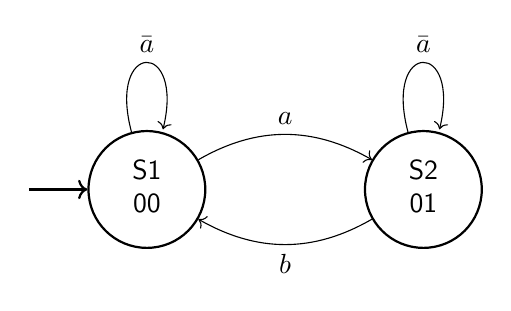
\begin{tikzpicture}[node distance=2cm,auto,every place/.style={draw}]
		\node [place] (S1) {\begin{tabular}{c}S1\\00\end{tabular}};
		\coordinate[node distance=1.5cm,left of=S1] (left-S1);
		\draw[->,thick] (left-S1) -- (S1);
		
		\node [place] (S2) [right=of S1] {\begin{tabular}{c}S2\\01\end{tabular}};
		\path[->] (S1) edge [bend left] node {$a$} (S2);
		\path[->] (S2) edge [bend left] node {$b$} (S1);
		\path[->] (S2) edge [loop above] node {$\bar{a}$} ();
		\path[->] (S1) edge [loop above] node {$\bar{a}$} ();
	\end{tikzpicture}	
	\centering
	\caption{Example single input state diagram}
\end{figure}
\textit{Note: I couldn't figure out how to add the line that is meant to go between the state label and the state number}

\subsubsection{Completeness}
Each possible combination of inputs should be addressed \textbf{exactly once} for each state. i.e. transition arrows from each state must encompass all possibilities (exactly once)

\subsection{State tables}
\begin{itemize}
	\item State diagrams can also be represented in a state table	
\end{itemize}

\begin{table}[H]
	\centering
	\caption{Example State Table}
	\begin{tabular}{cc|c|cc}
		\textbf{Current State} & \textbf{Input $U$} & \textbf{Next State} & \multicolumn{2}{c}{\textbf{Outputs}}\\
		&&& $Q_1$ & $Q_2$\\\hline
		S0 & 0 & S3 & 0 & 0\\
		S0 & 1 & S1 & 0 & 0\\
		S1 & 0 & S0 & 0 & 1\\
		S1 & 1 & S2 & 0 & 1\\
		S2 & 0 & S1 & 1 & 0\\
		S2 & 1 & S3 & 1 & 0\\
		S3 & 0 & S2 & 1 & 1\\
		S3 & 1 & S1 & 1 & 1
	\end{tabular}
\end{table}

\begin{table}[H]
	\centering
	\caption{Two-dimensional state table}
	\begin{tabular}{c|cc|cc}
		\textbf{Current} & \multicolumn{2}{c}{Next State} & \multicolumn{2}{c}{Outputs}\\
		\textbf{State} & $\bar{U}$ & $U$ & $Q_1$ & $Q_0$\\\hline
		S0 & S3 & S1 & 0 & 0\\
		S1 & S0 & S2 & 0 & 1\\
		S2 & S1 & S3 & 1 & 0\\
		S3 & S2 & S0 & 1 & 1
	\end{tabular}
\end{table}

\subsection{State encoding}
\begin{itemize}
	\item Must encode each state into flip-flop values
	\item Choose
	\subitem Number of flip-flops
	\subitem Bit patterns that represent each state
	\item Ideally, choose state encoding to make combinational logic simple, for both
	\subitem Output logic
	\subitem Next state logic	
\end{itemize}
\section{Visualising multidimensional data}
\subsection{Ternary plots}
\begin{itemize}
	\item Triangular ordination of \textit{proportions} of 3 components (i.e. $\sum=1$)
	\item tricky but worth the effort
	\item axes read parallel to each zero (center = 33\% each)	
\end{itemize}

\subsection{Scatterplot matrix}
\begin{itemize}
	\item tiled 2d visualisation of multiple variables
\end{itemize}

\subsection{Coplots}
\begin{itemize}
	\item conditional on one variable
	\subitem slice through data
	\subitem slices trade-off range and data
	\subitem fit curves to see dependency
	\subitem can also graph residuals etc.	
\end{itemize}

\subsection{3d point plots}
\begin{itemize}
	\item scatterplot in 3d
	\item used to seeing a 3d object in 2d
	\item if not too many points can use a stem plot	
\end{itemize}

\subsubsection{Interpolating}
\begin{itemize}
	\item if irregular x/y data
	\item create lattice covering range of x and y
	\item interpolate between z-values	
\end{itemize}

\subsubsection{viewing/presentation choices}
\begin{itemize}
	\item grid density
	\begin{itemize}
		\item sparse = lose surface definition
		\item dense = lose depth perception
	\end{itemize}
	\item axis ratios
	\begin{itemize}
		\item as data if axes share same units
		\item otherwise 1-1-1
		\item or banked z-axis?
	\end{itemize}
	\item projection
	\begin{itemize}
		\item perspective: good for real objects (but distortion)
		\item orthogonal: fixed lengths $\rightarrow$ data analysis (but front/back confusion)
	\end{itemize}
	\item orientation (azimuth and elevation)
	\begin{itemize}
		\item multiple rotations helpful (around z-axis, in equal steps)
	\end{itemize}
	\item other effects
	\begin{itemize}
		\item box
		\item ticks
		\item curtain
		\item show/hide rear wires
		\item colour
	\end{itemize}	
\end{itemize}
All involve trade-offs
\begin{itemize}
	\item help or hindrance
	\item should highlight data, not effect itself	
\end{itemize}

\subsubsection{colour representation}
use of colour
\begin{itemize}
	\item none
	\item height-related
	\item gradient-related	
\end{itemize}

\section{CPU Control Unit}
\subsection{Control Unit}
\begin{itemize}
	\item Control signals come from the \textbf{control unit}
	\item Control unit must generate the control signals in the right order for a given instruction
	\subitem Instruction determined by contents of the \textbf{Instruction Register (IR)}	
\end{itemize}

\subsubsection{Data Influencing Control}
\begin{itemize}
	\item Need to know more than what's in the instruction register
	\item Control unit can't operate without knowing something about the data
	\item \textbf{Status Register}
	\subitem Determined by ALU operations
	\subitem Stores status of last ALU operation	
\end{itemize}

\begin{note}{Status Register}
Typically Includes:
	\begin{description}
		\item[Z:] zero bit -- was the last result 0?
		\item[V:] overflow bit -- did the last addition/subtraction operation overflow (assuming it was a two's complement operation)?
		\item[C:] carry bit -- was a carry out generated?
		\item[N:] negative bit -- was the result negative if considered as two's complement (i.e. what's the sign bit)?
	\end{description}	
\end{note}
\section{Computer Graphics (CG)}
\subsection{What is CG}
\begin{itemize}
	\item Algorithms, Techniques, and Processes that
	\item Execute on computers (by definition)
	\item Produce images (of some description)
	\subitem On screens, in files, VR headsets, printers, t-shirts, or anything really
	\item Related (sometimes very closely) but \textit{not} CG as such
	\begin{itemize}
		\item Image processing
		\item Data acquisition / scanning
		\item Fabrication (e.g. 3d printing)
		\item Simulation
		\item Visualisation
	\end{itemize}	
\end{itemize}

\subsection{Offline}
Higher quality image or series of images. Can take hours to compute which is fine because there is no human interaction.
\begin{itemize}
	\item Frame time > 2 min
	\item Final image quality (render farms)
	\item Image stability (animation)
	\item Time to predictive image	
\end{itemize}

\subsection{Interactive}
\begin{itemize}
	\item 33ms - 1s/frame
	\item Performance (Special HW ok)	
\end{itemize}


\subsection{Real Time}
Main goal is to be interactive, so quality is a secondary concern.
\begin{itemize}
	\item <33ms / frame
	\item Single workstation performance
\end{itemize}

\subsection{VR / AR}
\begin{itemize}
	\item <10ms / frame
	\item Single workstation performance
	\item Stereo images
	\item Wide field of view
	\item Low latency
	\item Disparity
	\item Image stability
	\item Close range detail	
\end{itemize}

\section{Coordinate Systems}
\subsection{Euclidean Space}
Can be 2D or 3D and is defined as the ``normal space'', i.e. it behaves like the observable world. The space is made up of coordinates which are typically Cartesian

\subsection{Points and Vectors}
Point is a location or position, Vector has a direction and length (from two points)

\section{Transformations}
\begin{itemize}
	\item Position/Movement: \textbf{Translation}
	\item Orientation: \textbf{Rotation}
	\item Size: \textbf{Scale}
	\item Inverse	
\end{itemize}

\subsection{Translation}
\begin{itemize}
	\item Movement along a vector
	\item For all points in space:
	\subitem $P' = P + t$
	\subitem $T(t)$ denotes translation by vector $t$	
\end{itemize}

\subsection{Rotation}
\begin{itemize}
	\item Rotation in angles around a vector
	\item Rotation around $Y$ axis: $R_y(\alpha)$
	\item Rotation around arbitrary vector: $R(v,\alpha)$	
\end{itemize}

\subsection{Scale}
Uniform, $S(s)$:
\begin{itemize}
	\item Same in all axes
	\item For all points: $P' = sP$	
\end{itemize}
Non-Uniform, $S(v)$:
\begin{itemize}
	\item Different value for $x,y,z$
	\item For all points: $P' = vP$	
\end{itemize}

\subsection{Handedness}
\begin{itemize}
	\item Affects rotations
	\item Affects back-face culling
	\item A model is authored for LH or RH
	\subitem Mirrored if viewed in opposite
	\item Conversion \textit{can} be tricky	
\end{itemize}


\section{Spaces}
% !TeX spellcheck = en_US
% !TeX root = notes.tex
\subsection{Multimedia}
\subsubsection{Audio}
\begin{itemize}
	\item Analog audio signal sampled at constant rate (telephone: 8000 samples/sec, CD music: 44,100 samples/sec)
	\item quantized, i.e. rounded (8 bits for 256 values)
	\item Example rates (CD: 1.411 Mbps, MP3: 96,128,160 kbps, Internet Telephony: 5.3 kpbs)
\end{itemize}
\subsubsection{Video}
\begin{itemize}
	\item MPEG 1 (CD-ROM) 1.5 Mbps
	\item MPEG 2 (DVD) 3-6 Mbps
	\item MPEG 4 (often used in Internet) <1 Mbps
\end{itemize}
\subsubsection{3 Application Types}
\begin{itemize}
	\item\textbf{Streaming, stored} audio, video
	\begin{description}
		\item[streaming:] can begin playout before downloading entire file
		\item[stored (at server):] can transmit faster than audio/video will be rendered (implies storing/buffering at client)
	\end{description}
	\item\textbf{conversational} voice/video over IP (interactive nature of human-to-human conversation limits delay tolerance
	\item\textbf{streaming live} audio, video
	\item Once playout begins, playback must match original timing (network delays are variable)
	\begin{itemize}
		\item\textbf{Client-side buffer} to match playout requirements
	\end{itemize}
	\item RTP [RFC 2326] multimedia payload types
\end{itemize}

\subsection{Voice-over-IP (VoIP)}
\begin{itemize}
	\item\textbf{VoIP end-end-delay requirement:} needed to maintain ``conversational'' aspect (< 150msec: good, > 400msec bad)
	\item\textbf{session initialization:} how does callee advertise IP address, port number, encoding algorithms?
	\item\textbf{value-added services:} call forwarding, screening, recording
	\item\textbf{emergency services:} 911
	\item\textbf{network loss:} IP datagram lost due to network congestion (router buffer overflow)
	\item\textbf{delay loss:} IP datagram arrives too late for playout at receiver
	\item\textbf{loss tolerance:} depending on voice encoding, loss concealment, packet loss rates between 1\% and 10\% can be tolerated
\end{itemize}
\subsubsection{Adaptive playout delay}
\begin{itemize}
	\item estimate network delay, adjust playout delay at beginning of each talk spurt
	\item silent periods compressed and elongated
\end{itemize}
$$ d_i = (1-\alpha)d_{i-1}+\alpha(r_i-t_i) $$
\begin{description}
	\item[$d_i$:] delay estimate after ith packet
	\item[$\alpha$:] small constant e.g. 0.1
	\item[$r_i$:] time received
	\item[$t_i$:] time sent (timestamp)
\end{description}
\subsubsection{Recovery from packet loss}
\textbf{simple FEC (Forward Error Correction)}
\begin{itemize}
	\item for every group of $n$ chunks, create redundant chunk by exclusive OR-ing $n$ original chunks
	\item send $n+1$ chunks, increasing bandwidth by factor $\frac{1}{n}$
	\item can reconstruct original $n$ chunks if at most one lost chunk from $n+1$ chunks, with playout delay
\end{itemize}
%\subsubsection{Skype}
%\begin{leftbar}
%	Proprietary application-layer protocol (inferred via reverse engineering) $\rightarrow$ encrypted messages
%\end{leftbar}
%\begin{figure}[H]
%	\includegraphics[width=\linewidth]{skype}
%	\centering
%	\caption{Skype Network Layout}
%\end{figure}
%P2P components:
%\begin{description}
%	\item[clients:] Skype peers connect directly to each other for VoIP call
%	\item[super nodes (SN):] Skype peers with special functions
%	\item[overlay network:] among SNs to locate SCs
%	\item[login server]
%\end{description}

\subsection{Real-Time Protocol (RTP)}
\begin{itemize}
	\item RTP specifies packet structure for packets carrying audio, video data
	\item RFC 3550
	\item RTP packet provides
	\begin{itemize}
		\item payload type identification
		\item packet sequence numbering
		\item time stamping
	\end{itemize}
	\item RTP runs in end systems
	\item RTP packets encapsulated in UDP segments
	\item interoperability: if two VoIP applications run RTP, they may be able to work together
\end{itemize}
\subsubsection{RTP runs on top of UDP}
RTP libraries provide transport-layer interface that extends UDP:
\begin{itemize}
	\item port numbers, IP addresses
	\item payload type identification
	\item packey sequence numbering
	\item time-stamping
\end{itemize}
\subsubsection{RTP and QoS}
\begin{itemize}
	\item RTP does \textbf{not} provide any mechanism to ensure timely data delivery or other QoS guarantees
	\item RTP encapsulation only seen at end systems (not by intermediate routers)
	\subitem routers provide best-effort service, making no special effort to ensure that RTP packets arrive at destination in timely matter
\end{itemize}

\subsection{Real-Time Control Protocol (RTCP)}
\begin{itemize}
	\item works in conjuncation with RTP
	\item each participant in RTP session periodically sends RTCP control packets to all other participants
	\item each RTCP packet contains sender and/or receiver reports
	\subitem report statistics useful to application: \# packets sent, \# packets lost, interarrival jitter
	\item feedback used to control performance
	\subitem sender may modify its transmissions based on feedback
\end{itemize}
\subsubsection{RTCP: packet types}
\begin{description}
	\item[receiver report packets:] fraction of packets lost, last sequence number, average interarrival jitter
	\item[sender report packets:] SSRC of RTP stream, current time, number of packets sent, number of bytes sent
	\item[source description packets:] email address of sender, sender's name, SSRC of associated RTP stream. Provide mapping between the SSRC and the user/host name
\end{description}

\subsection{SIP: Session Initiation Protocol}
\textbf{long-term vision:}
\begin{itemize}
	\item all telephone calls, video conference calls take place over Internet
	\item people identified by names or e-mail addresses, rather than by phone numbers
	\item can reach callee (if callee so desires), no matter where callee roams, no matter what IP device callee is currently using
\end{itemize}
\subsubsection{SIP services}
\begin{itemize}
	\item SIP provides mechanisms for call setup:
	\begin{itemize}
		\item for caller to let callee know she wants to establish a call
		\item so caller, callee can agree on media type, encoding
		\item to end call
	\end{itemize}
	\item determine current IP address of callee: maps mnemonic identifier to current IP address
	\item call management:
	\begin{itemize}
		\item add new media streams during call
		\item change encoding during call
		\item invite others
		\item transfer, hold calls
	\end{itemize}
\end{itemize}
\textit{SIP default port 506}\\
\textbf{SIP registrar}\\
Function of SIP server (registrar). When Bob starts SIP client, client sends SIP REGISTER message to Bob's registrar server\\
\textbf{SIP proxy}\\
Function of SIP server (proxy). Alice sends invite message to her proxy, proxy responsible for routing SIP messages to callee possibly through multiple proxies. Bob sends response back through same set of SIP proxies, proxy returns Bob's SIP response message to Alice. SIP proxy analogous to local DNS server plus TCP setup

\begin{note}{Comparison with H.323}
	\begin{itemize}
		\item Another signaling protocol for real-time, interactive multimedia
		\item Complete, vertically integrated suite of protocols for multimedia conferencing; signaling, registration, admission control, transport, codecs
		\item SIP is a single component. Works with RTP, but does not mandate it. Can be combined with other protocols, services
		\item SIP uses KISS principle
	\end{itemize}
\end{note}
% Just a bunch of basic C, basically arrays, pointers, memory, preprocessor stuff
\begin{note}{AVR Status Bit}
	\begin{itemize}
		\item $N$ bit $=$ negative (1 if sign bit of result is 1)
		\item $V$ bit $=$ two's complement overflow
		\item $S=N\oplus V$	
	\end{itemize}
	If overflow happens, sign bit will be wrong so instead of checking $N$ bit, check $S$ bit
\end{note}

\section{Flow of Control}
\subsection{Procedures}
\begin{itemize}
	\item Group of instructions that performs some task
	\item May have operands (\textbf{arguments} or \textbf{parameters})
	\item May produce result(s)
	\item Can be \textbf{invoked} (called) from multiple places in program
	\item After invocation, control returns to the statement after the call
	\item Also known as a \textbf{subroutine, function, method}	
	\item Return address is stored in a stack
\end{itemize}

\section{Interrupts}
CPU receiving interrupt causes it to execute software to handle the interrupt
\begin{itemize}
	\item Software routine is called \textbf{interrupt handler} or \textbf{interrupt service routine (ISR)}
\end{itemize}

\subsection{Finding the Interrupt Handler}
Look in the \textbf{interrupt vector table} which contains either a table of addresses or table of jump instructions

\subsubsection{Transparency}
When ISR finishes, computer is in the same state as it was before the interrupt. Save the status register and any other registers that will be used by the interrupt.

\subsubsection{Interrupt Priority}
Priority only occurs when two priorities are triggered at relatively the same time. Highest priority is the one with the lower vector value

\subsection{Traps}
Traps are \textbf{software interrupts} caused by events in software.
\begin{itemize}
	\item Overflow, Divide by zero, Undefined opcode
	\item Traps save continually checking for errors
	\item Trap handlers (service routines) don't always return to the original program
\end{itemize}

\section{Pulse Width Modulation (PWM)}
\begin{description}
	\item[Duty cycle:] \% of time that the signal is high
	\item[Average Value:] If the periodic pulse is fast enough, signal looks like the average value (brightness control of led)
	\item[Fast PWM Mode:] Output is high on \texttt{OCR0B} trigger and low (and reset) on \texttt{OCR0A} trigger
	\item[Phase Correct PWM:] Center of pulses remain the same point in period. Counter counts up and then down
\end{description}
\section{Serial}
\subsection{Synchronous}
\textbf{SPI} - Serial Peripheral Interface

\subsection{Asynchronous}
\textbf{UART} - Universal Asynchronous Receiver and Transmitter\\
\textbf{USART} - Universal Synchronous/Asynchronous Receiver and Transmitter\\
\textbf{USB} - Universal Serial Bus

\begin{note}{Sync vs Async}
	\begin{description}
		\item[Sync:] Clock signal is transmitted with data
		\item[Async:] Clock signal must be recovered from data stream
		\subitem Example: Use start and stop bits
	\end{description}
\end{note}

\subsubsection{Baudrate}
Symbols per second. Not the same as bit rate. 2400, 4800, 9600, 14400, 19200, 28800, 38400, 57600, 115200

\begin{align*}
	\texttt{UBRRn} &= \frac{f_{\texttt{OSC}}}{16\times \texttt{BAUD}} - 1
	&= \frac{8\times10^6}{16\times\texttt{BAUD}} - 1	
\end{align*}

\section{Analog to Digital Conversion (ADC)}
Input pin is compared against GND and a reference voltage (VREF)
\subsection{Bus Masters and Slaves}
\textbf{Master} - Device which initiates (and controls) the transfer of data\\
\textbf{Slave} - Waits for requests, responds to master
\textbf{I\textsuperscript{2}C} - Inter-Integrated Circuit
\textbf{TWI} - Two-wire Interface
\textbf{1-Wire} - Communication over a single wire
\textbf{Bit Bashing} - Simulate I/O standards with general purpose ports
\input{lec20}
\section{Assembly}
Statements have 4 parts:
\begin{description}
	\item[Labels] needed so statements can be jumped to, and so that data can be referenced
	\item[Opcode] has symbolic abbreviation for an instruction opcode
	\item[Operand] field specifies addresses and registers used as operands of the instruction
	\item[Comments] field is space for programmer to put helpful explanations
\end{description}
A command (directive) to the assembler itself! Preceded with a ``.'', called \textbf{Pseudo-instruction} or \textbf{directive}

\subsection{Memory Segments}
\begin{itemize}
	\item Different types of memory are known as \textbf{segments} to the assembler
	\item Assembler directives enable code/data to be placed into different segments
	\item AVR has
	\begin{itemize}
		\item Data segment (RAM)
		\subitem Can't place values here, just reserve space (for variables)
		\item Code segment (Flash)
		\subitem Can place program code or constant data here
		\item EEPROM Segment	
		\subitem Can place constants here
	\end{itemize}
\end{itemize}

\subsection{Pseudo-instructions}
\begin{itemize}
	\item \texttt{.byte}: Reserve space; only allowed in \textbf{dseg} (RAM)
	\item Segment directives \texttt{.cseg} and \texttt{.dseg} allow the text and data segments to be built up in pieces
	\item \texttt{.db}: Initialise constant in code or EEPROM segment
	\item \texttt{.dw}: As above but defines a 16-bit word
	\item \texttt{.def}: Make a definition (for registers only)
	\item \texttt{.device}: Specify the exact processor that this program is designed for (\texttt{.device ATmega324A})
	\item \texttt{.include}: Include a file
	\item \texttt{.exit}: Stop processing this file
	\item \texttt{.equ}: Equate (not changeable)
	\item \texttt{.set}: Equate (but changeable)
	\item \texttt{.org}: Set location counter - i.e. address (in any segment)
\end{itemize}

\section{Compiling and Linking}
\subsection{Object File Structure}
\begin{description}
	\item[6. End of module:] Contains address at which to start execution and maybe a checksum
	\item[5. Relocation dictionary:] Contains: List of addresses of code/data in (4) that need to be relocated
	\item[4. Machine instructions and constants:] Contains: Assembled code and constants (code segment, data segment)
	\item[3. External reference table:] Contains: List of all symbols that are used in the module but not defined in module
	\item[2. Entry point table:] Contains: List of symbols other modules can reference. Values of symbols (addresses): Procedure entry points, variables, addresses are relative to beginning of this object module
	\item[1. Identification:] Contains: Name of module, Location of the other sections in the file, Assembly date
\end{description}

\subsection{Dynamic Linking}
Linking can happen at run-time. Link when the procedure is first called. DLLs on Windows, SO on *nix. Advantages:
\begin{itemize}
	\item Saves space, libraries aren't linked into binary executable
	\item Library can be updated independently of the programs that use it, can be disadvantage also
\end{itemize}

\section{Memory and Disks}
\subsection{Memory Types}
\begin{description}
	\item[Static] memory: Flip-flops or latches used to store bits
	\item[Dynamic] memory: Each cell is a switch (transistor) plus capacitor
	\item[RAM]: Volatile read/write memory
	\item[SRAM]: Static memory
	\item[DRAM]: Dynamic memory
\end{description}

\subsection{Volatility}
\textbf{Volatile memory}
\begin{itemize}
	\item Contents ``forgotten'' when power off
	\item Both SRAM and DRAM are volatile
	\subitem DRAM forgets contents within milliseconds if not refreshed, i.e. contents rewritten	
\end{itemize}
\textbf{Non-volatile memory}
\begin{itemize}
	\item Contents remembered when power off	
	\item \textbf{ROM} - Read only memory
	\item \textbf{EPROM} - Erasable Programmable ROM
	\item \textbf{EEPROM} - Electronically Erasable PROM
	\item \textbf{Flash} - New EEPROM
\end{itemize}

\begin{note}{When do use powers of 2 or 10}
	\begin{itemize}
		\item \textbf{Main Memory} capacity, always 	based on powers of 2
		\subitem $1GB=1024\times1024\times1024 bytes = 2^{30} bytes$
		\item \textbf{Hard Disks}, manufacturers base sizes on powers of 10
		\subitem $1GB = 1000\times1000\times1000 bytes=10^9bytes$
		\subitem Operating Systems base sizes on powers of 2
		\item \textbf{Data Speeds (transfer rates)} based on powers of 10
		\subitem $1Gbps = 10^9 bits per second$
	\end{itemize}
\end{note}

\subsection{Kibibytes, Mebibytes}
\begin{itemize}
	\item Kilo-, mega-, giga- prefixes mean powers of 10 in SI units
	\item 1 \textbf{kibibyte} = 1KiB = 1024 bytes
	\item 1 \textbf{mebibyte} = 1MiB = 1024 KiB
	\item 1 \textbf{gibibyte} = 1GiB = 1024 MiB	
\end{itemize}

\subsection{Types of DRAM}
\begin{itemize}
	\item Bits stored as charge on capacitor, not in flip-flops
	\item Cells are smaller, so can pack more bits on a chip than static memory
	\item Fast Page Mode (FPM DRAM)
	\item Extended Data Out (EDO DRAM)
	\item Synchronous DRAM (SDRAM)
	\item Rambus DRAM (RDRAM)
	\item Double Data Rate DRAM (DDR DRAM) 1, 2, 3, and 4	
\end{itemize}

\subsection{Cache Memory}
\begin{itemize}
	\item CPUs are faster than main memory
	\item Small amount of very fast memory combined with larger slower memory
	\item Most commonly used memory words kept in cache
	\item Three levels, each lower is progressively slower but larger	
\end{itemize}

\subsection{Magnetic Disks}
\begin{itemize}
	\item Rotating \textbf{platters} with magnetised coating
	\item Data stored magnetically in circular \textbf{tracks}
	\item Read/write \textbf{heads} float above platter surfaces
	\item Usually use both sides of platters	
\end{itemize}

\subsubsection{Sectors and Tracks}
\begin{figure}
	\centering
	\includegraphics[width=0.8\linewidth]{disk}
	\caption{The break up of what a disk is}
\end{figure}

\subsubsection{Cylinders}
\begin{itemize}
	\item Set of tracks at a given radial position
	\item Number of tracks in cylinder = 2 x number of platters
\end{itemize}

\subsubsection{Sectors}
\begin{itemize}
	\item Tracks divided into fixed-length sectors
	\subitem Smallest data unit, i.e. must read/write a whole sector at a time
	\item Sector consists of: Preamble, Data, Error correction codes (ECCs), Inter-sector gap
	\item About 85\% of disk capacity usable by operating system	
\end{itemize}

\subsubsection{Access Time}
\begin{itemize}
	\item \textbf{Access Time} = seek time + rotational latency + transfer time
	\item \textbf{Seek time} - time to move heads to right cylinder
	\item \textbf{Rotational latency} - time to wait for sector to arrive under head
	\item \textbf{Transfer time} - Time for sector to pass under	
\end{itemize}

What's the average access time for a hard dick which rotates at 7200rpm and has an edge-to-edge seek time of 10ms? (Assume that seek time is proportional to the number of tracks to seek)
\begin{align*}
	\text{Avg Access Time} &= \text{Avg seek time} + \text{Avg rotational}\\
	&= \frac{\text{e-to-e seek}}{3} + \frac{\text{rot time}}{2}\\
	&= \frac{10}{3} + \frac{1/120}{2}\\
	&= 7.5ms
\end{align*}



\section{File Systems, Buses and Chipsets}
\subsection{File System}
FAT, FAT32, NTFS, exFAT, EXT2, EXT3, EXT4, APFS, HFS+, UFS, ZFS
\begin{itemize}
	\item Some sectors used for index information (e.g. File Allocation Table)	
\end{itemize}
\subsubsection{Disk Formatting}
\begin{itemize}
	\item\textbf{Low level format} - Reinitialises all sectors
	\item\textbf{High level format} - Creates empty file system, only writes index/table sectors	
\end{itemize}

\begin{note}{Fragmentation}
	The sectors on the disk become non-contiguous leaving the disk with unused sectors resulting in a slower access due to seek time.	
\end{note}

\subsection{Buses}
Bus controller is know a \textbf{chipset}. DDR4-RAM, DDR3, PCI Express, USB, SATA, PCI. \textbf{Peripheral} bus is an external I/O device.

\subsubsection{PCI Bus}
\begin{itemize}
	\item Peripheral Component Interconnect bus
	\item PCI 1 - 32 bits wide, 33 MHz, 132MB/sec
	\item PCI 2.2 - 64bit wide, 66MHz, 528MB/sec
	\item 32bit cards have 120 pins
	\item 64bit cards have an extra 64-bit connector	
\end{itemize}




\section{Floating Point Numbers}
\begin{itemize}
	\item Single Precision (32 bits)
	\subitem 1 sign bit, 8 exponent (excess 127 format), 23 mantissa
	\item Double Precision (64 bits)
	\subitem 1 sign bit, 11 exponent (excess 1023), 52 mantissa	
\end{itemize}
\begin{align*}
	-23.25 &= -(16 + 4 + 2 + 1 + 0.25)\\
	&= -10111.01000....\\
	&= -1.011101000\times2^4\\
	&= [1][10000011][0111010000...00]	
\end{align*}

\section{Pipelining}
Allows the processor to fetch and execute code ahead of time
\begin{itemize}
	\item\textbf{Higher clock rate} (i.e. reduced clock cycle time)
	\subitem Maximum clock rate determined by most complex logic path in circuit
	\item\textbf{Higher throughput} more instructions executed per unit time
	\subitem Achieve one instruction per cycle (if pipeline is full)	
\end{itemize}


\end{multicols}
\end{document}
